\section{Pruning and enrichment}
For long chains the RR algorithm becomes inefficient and inaccurate, as was shown by Batoulis and Kremer \cite{batoulis1988statistical}. The inefficiency occurs due to the fact that still too much time is spent on generating polymers with a low Boltzmann weight. The inaccuracy is caused due to the fact that the weights of the individual monomers are only weakly correlated, which results in a large spread in the final weights of the polymers. This causes a few configurations to dominate the distribution, causing those configurations to dominate the ensemble average. 

To sample the phase space more effectively, Grassberger has suggested pruning and enriching the population. If a partially grown polymer gets a weight below a certain threshold, half of the time the polymer is discarded (`pruned'), and the other half of the time its weight is doubled (to compensate for the pruned polymers) and growing continues. The is done to compensate for changes in the distribution due to removing polymers. When a partially grown polymer gets a weight above a certain threshold, the polymer is split. Both polymers are independently grown from this point on and their weights are halved. The population is now `enriched'. This combined with the RR algorithm is called the pruned-enriched Rosenbluth method (PERM). 

The reasoning behind pruning and enrichment is that it is inefficient to continue growing a partial polymer with a low weight since it will have a low contribution to the weighted average. It is then better to prune this polymer and start over. When a polymer gets a relatively high weight it is important and advantageous to make a copy of this polymer.

\begin{Figure}
    \vspace{18 mm}
    \centering
    \def\svgwidth{\linewidth}
    %% Creator: Inkscape inkscape 0.48.3.1, www.inkscape.org
%% PDF/EPS/PS + LaTeX output extension by Johan Engelen, 2010
%% Accompanies image file 'perm.eps' (pdf, eps, ps)
%%
%% To include the image in your LaTeX document, write
%%   \input{<filename>.pdf_tex}
%%  instead of
%%   \includegraphics{<filename>.pdf}
%% To scale the image, write
%%   \def\svgwidth{<desired width>}
%%   \input{<filename>.pdf_tex}
%%  instead of
%%   \includegraphics[width=<desired width>]{<filename>.pdf}
%%
%% Images with a different path to the parent latex file can
%% be accessed with the `import' package (which may need to be
%% installed) using
%%   \usepackage{import}
%% in the preamble, and then including the image with
%%   \import{<path to file>}{<filename>.pdf_tex}
%% Alternatively, one can specify
%%   \graphicspath{{<path to file>/}}
%%
%% For more information, please see info/svg-inkscape on CTAN:
%%   http://tug.ctan.org/tex-archive/info/svg-inkscape
%%
\begingroup%
  \makeatletter%
  \providecommand\color[2][]{%
    \errmessage{(Inkscape) Color is used for the text in Inkscape, but the package 'color.sty' is not loaded}%
    \renewcommand\color[2][]{}%
  }%
  \providecommand\transparent[1]{%
    \errmessage{(Inkscape) Transparency is used (non-zero) for the text in Inkscape, but the package 'transparent.sty' is not loaded}%
    \renewcommand\transparent[1]{}%
  }%
  \providecommand\rotatebox[2]{#2}%
  \ifx\svgwidth\undefined%
    \setlength{\unitlength}{1006.82945118bp}%
    \ifx\svgscale\undefined%
      \relax%
    \else%
      \setlength{\unitlength}{\unitlength * \real{\svgscale}}%
    \fi%
  \else%
    \setlength{\unitlength}{\svgwidth}%
  \fi%
  \global\let\svgwidth\undefined%
  \global\let\svgscale\undefined%
  \makeatother%
  \begin{picture}(1,0.44813945)%
    \put(0,0){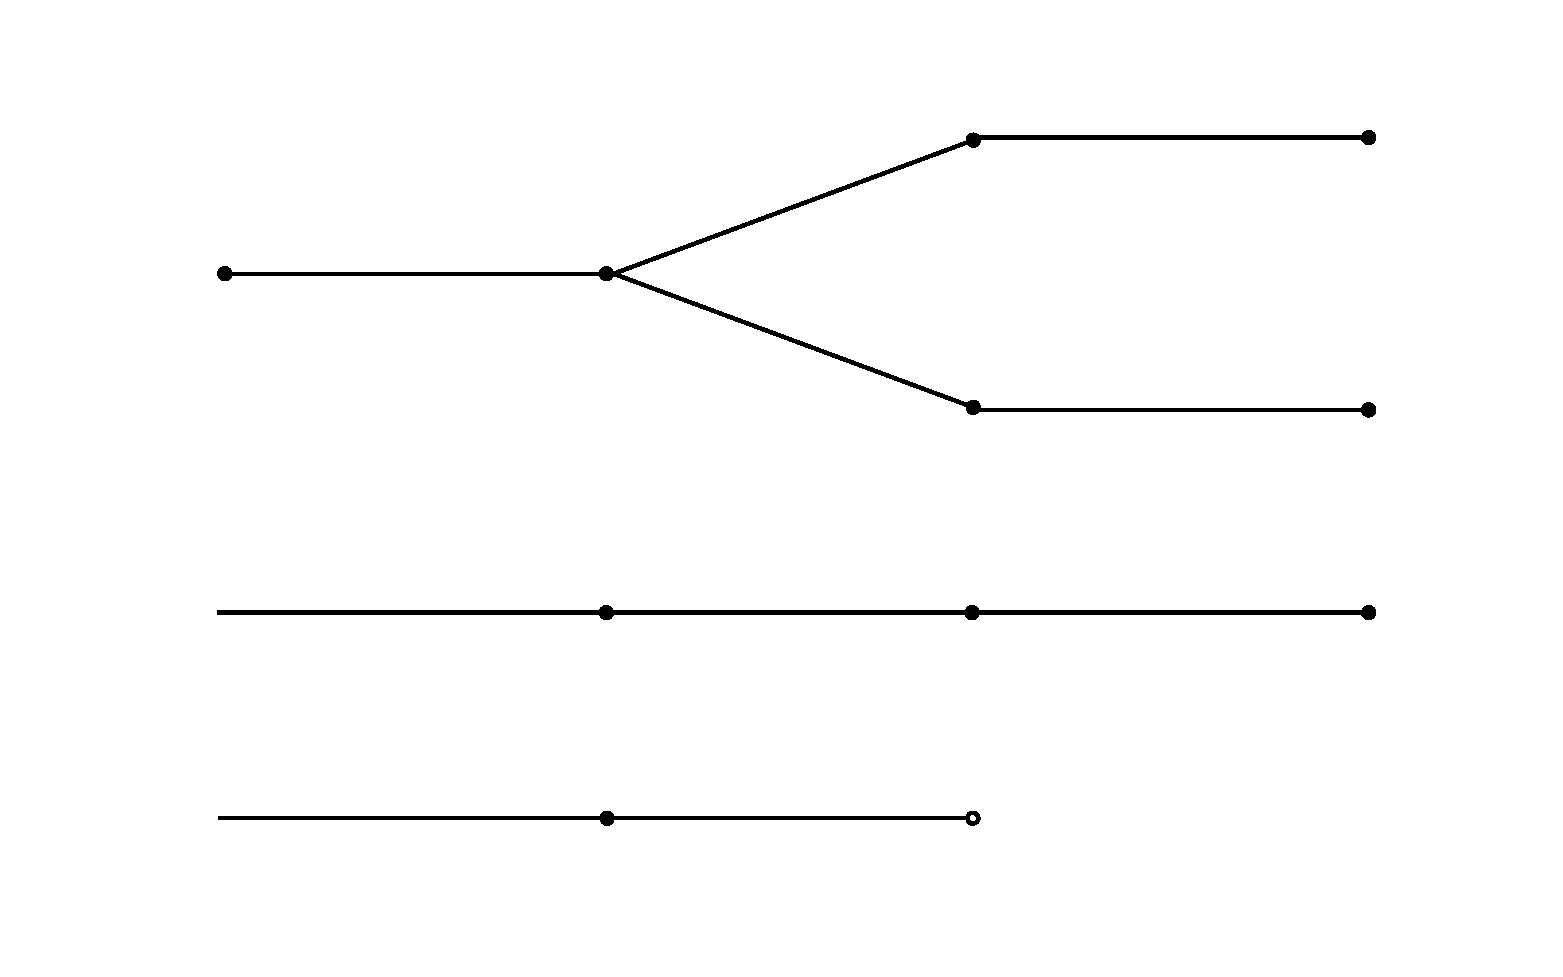
\includegraphics[width=\unitlength]{perm.eps}}%
    \put(0.69,0.56){\color[rgb]{0,0,0}\makebox(0,0)[lb]{\smash{$1/2\cdot W_n^{(l)}$}}}%
    \put(0.69,0.38){\color[rgb]{0,0,0}\makebox(0,0)[lb]{\smash{$1/2\cdot W_n^{(l)}$}}}%
    \put(0.69,0.25){\color[rgb]{0,0,0}\makebox(0,0)[lb]{\smash{$2\cdot W_n^{(l)}$}}}%
    \put(0.49,0.25){\color[rgb]{0,0,0}\makebox(0,0)[lb]{\smash{$c<1/2$}}}%
    \put(0.49,0.116){\color[rgb]{0,0,0}\makebox(0,0)[lb]{\smash{$c>1/2$}}}%
  \end{picture}%
\endgroup%

    \captionof{figure}{Pruning and enrichment. The new weights are depicted above each branch. $c$ is a random generated number between 0 and 1. Upper branch: the weight of the partial polymer $W_n^{(l)} > W_+^{(l)}$, so the polymer is split and the weight of both polymers is halved. The middle branch: $W_n^{(l)} < W_-^{(l)}$ and $c<1/2$ so the weight is doubled and the polymer continues growing. Bottom branch: $W_n^{(l)} < W_-^{(l)}$ and $c>1/2$ so the polymer is pruned.}
    \label{fig:perm}
\end{Figure}

For a finite system the partition sum can be estimated\cite{hsu2011review} by 
\begin{gather*}
    Z^{(l)} \simeq \hat{Z}^{(l)}
    = \frac{1}{N_l} \sum_{n=0}^{N_l}W_n^{(l)},
\end{gather*} where $N_l$ is the number of thus far completed polymers. The partition function is used to determine the upper limit $W_n^+$ and lower limit $W_n^-$ for the polymer weights, above or below which a polymer is enriched or pruned respectively as described by Hsu and Grassberger\cite{hsu2011review}. This is done as follows
\begin{gather*}
    W_+^{(l)} = C_+\hat{Z}^{(l)},\\
    W_-^{(l)} = C_-\hat{Z}^{(l)},
\end{gather*} where $C_+$ and $C_-$ are constants of order unity and should have a ratio $C_+/C_- \simeq \mathcal{O}(10)$. These constants determine if the population will grow or shrink and are chosen by running the simulation with different values and choosing the best combination.Figure \ref{fig:perm} shows an illustration of PERM.

For the first polymer there are no $\hat{Z}^{(l)}$ yet, so for this polymer the upper and lower limits are set to infinity and zero respectively ($ W_+^{(l)}= \infty$ and $W_-^{(l)}=0$). Resulting in the regular RR algorithm.

% The expectation value of a physical quantity $A$ can be determined by 
% \begin{equation}
%     \langle A \rangle^{(l)} = \frac{\sum_{n=0}^{N_l}A_nW_n^{(l)}}{\sum_{n=0}^{N_l}W_n^{(l)}}.
% \end{equation}
